%%%%%%%%%%%%%%%%%%%%%%%%%%%%%%%%%%%%%%%%%%%%%%%%%%%%%%%%%%%%%%%%%%%%%%%
%%%%  Load the document class and packages                         %%%%
%%%%%%%%%%%%%%%%%%%%%%%%%%%%%%%%%%%%%%%%%%%%%%%%%%%%%%%%%%%%%%%%%%%%%%%
\documentclass[a4paper]{report}
\usepackage{epsfig}            % to insert PostScript figures
\graphicspath{ 
  {figures/} 
}

%Change figure names
\renewcommand{\figurename}{Fig}

\usepackage[bf,footnotesize]{caption} % make captions small and label bold


\addtocounter{chapter}{1} %Because starting at zero is silly
\makeatletter
\renewcommand{\thesection}{\@arabic\c@section}
\renewcommand{\thefigure}{\@arabic\c@figure}
\makeatother

\usepackage[a4paper,margin=2.7cm,tmargin=2.5cm,bmargin=2.5cm]{geometry} 
\usepackage{textcomp}          % To make nice degree symbols and others\usepackage[bf,footnotesize]{caption} % make captions small and label bold
\usepackage{wrapfig}
%to produce the clickable references along the left in Acroread. This
%package must be included last. 
\usepackage[ps2pdf,bookmarks=TRUE]{hyperref} 



%%%%%%%%%%%%%%%%%%%%%%%%%%%%%%%%%%%%%%%%%%%%%%%%%%%%%%%%%%%%%%%%%%%%%%%
%%%%  Hypertext references for Acrobat                             %%%%
%%%%%%%%%%%%%%%%%%%%%%%%%%%%%%%%%%%%%%%%%%%%%%%%%%%%%%%%%%%%%%%%%%%%%%%
\hypersetup{
pdfauthor = {TENSS},
pdftitle = {Optics Exercises},
pdfkeywords = {optics, lenses, refraction, reflection, dispersion,
  telescope, microscope},
pdfcreator = {LaTeX with hyperref},
pdfproducer = {dvips + ps2pdf}
           }


\begin{document}




%set the number of sectioning levels 
\setcounter{secnumdepth}{2}

\begin{center}
\textbf{\Large{Optics Bench Exercises}}
\end{center}

\section{Introduction}
These exercises are designed to teach the basic principles of optics and image formation
\footnote{This document was originally written by Francesca Anselmi for a CSHL graduate course.
It was then modified for use at TENSS (www.tenss.ro) by Priyanka Gupta and Adriana Dabacan. 
The present version was created in 2018 by Rob Campbell for an imaging course at the Sainsbury Wellcome Centre, UCL.}.
The goal of the exercises is to nurture an understanding of image formation, conjugate planes, and how multiple lenses interact in simple optical set ups. 
It is helpful to have the free \textbf{ray optics simulator} from the Google Play store running on a computer when going through the exercises. 


\section{Equipment usage notes}
The black post holders mount to the rail carriages via a short cap screw as shown in Fig.~\ref{fig:post}. 
The carriages can then be attached to the rail, on which they can slide up and down. 
Use the lens tool to secure lenses in lens holders. 
`SM2' refers to two inch optics and associated accessories. 
`SM1' refers to one inch optics and associated accessories. 

\begin{figure}[h]
\center
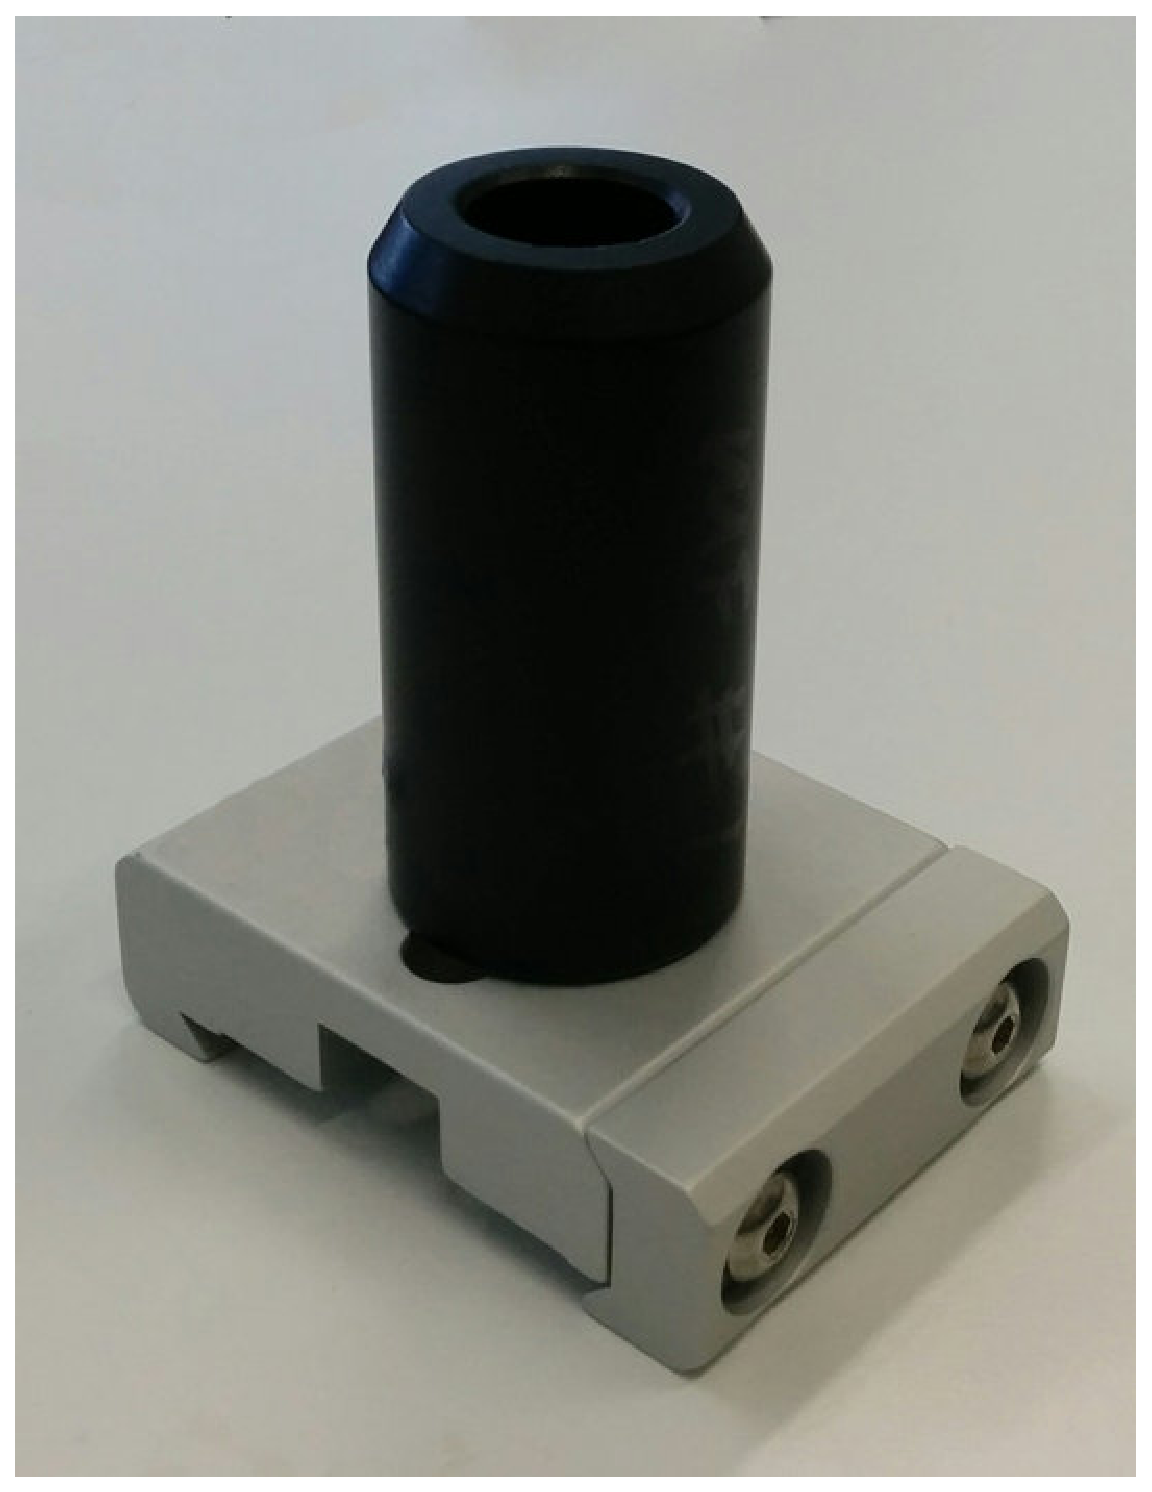
\includegraphics[width=1.3in]{post_mounted.eps}
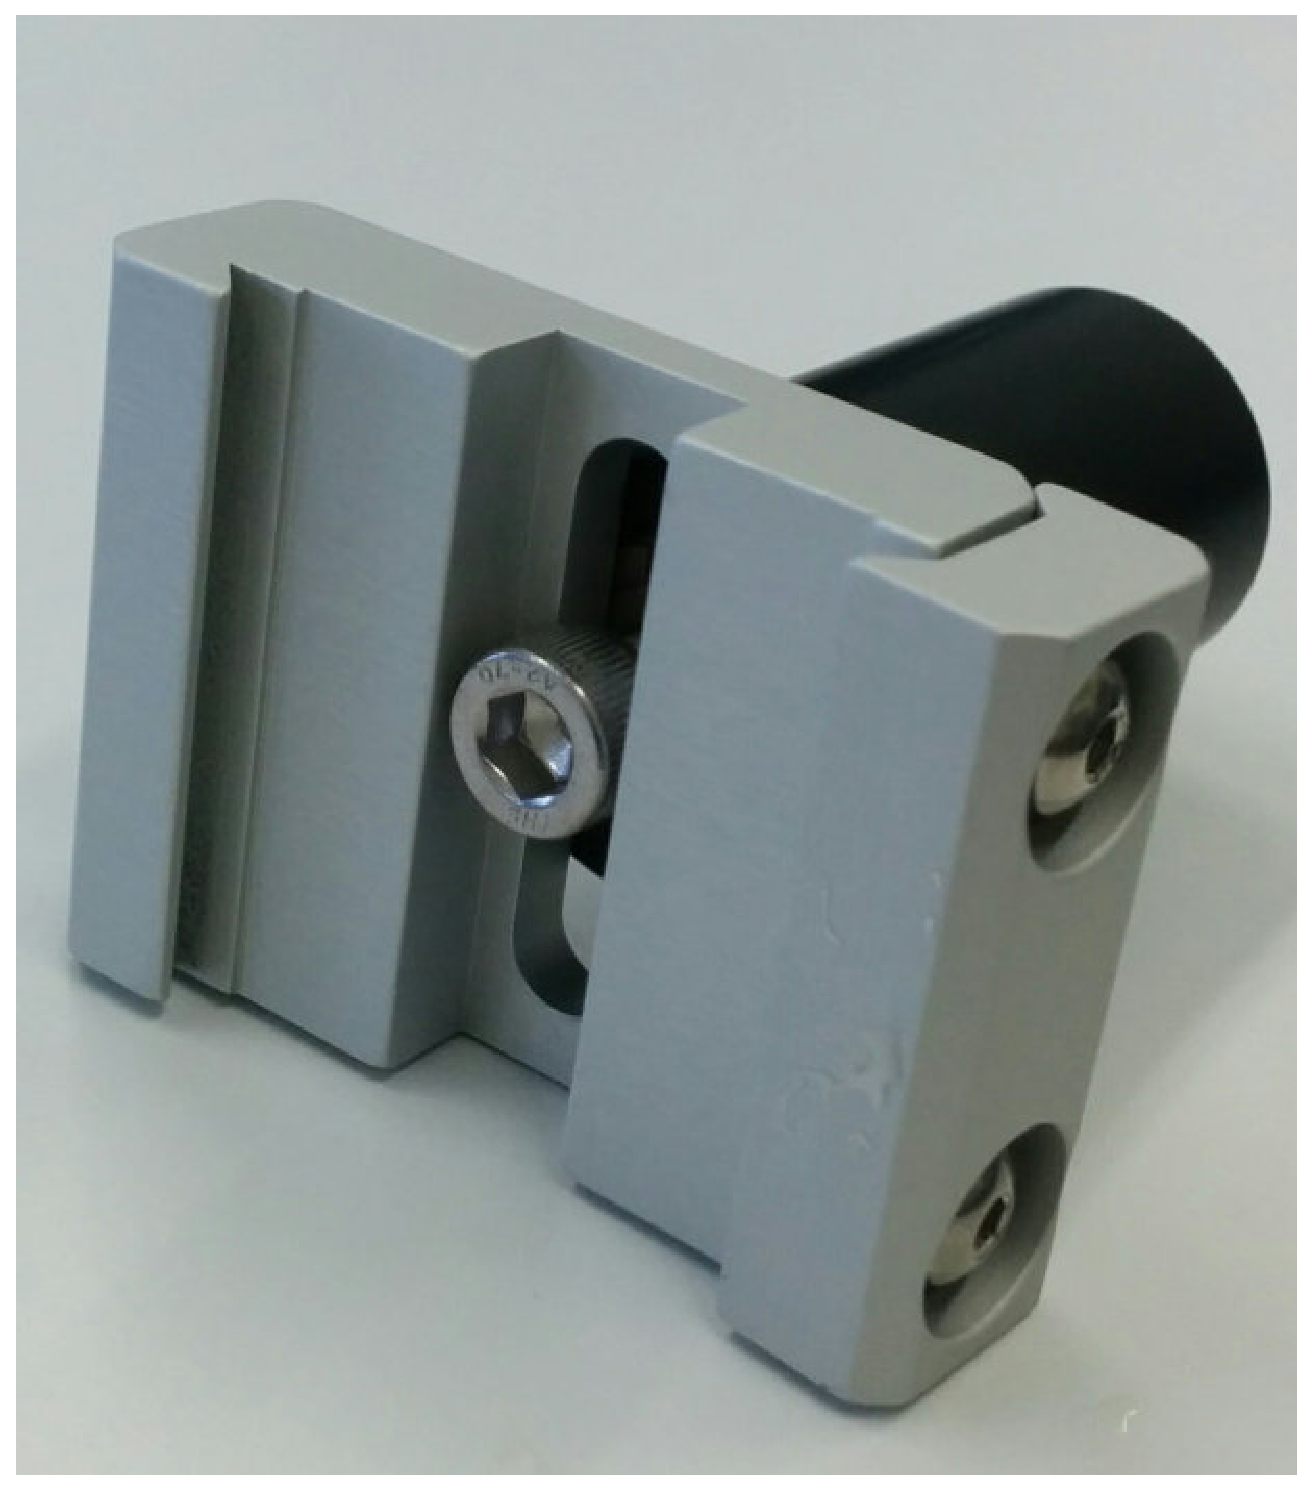
\includegraphics[width=1.5in]{post_mounted_underside.eps}
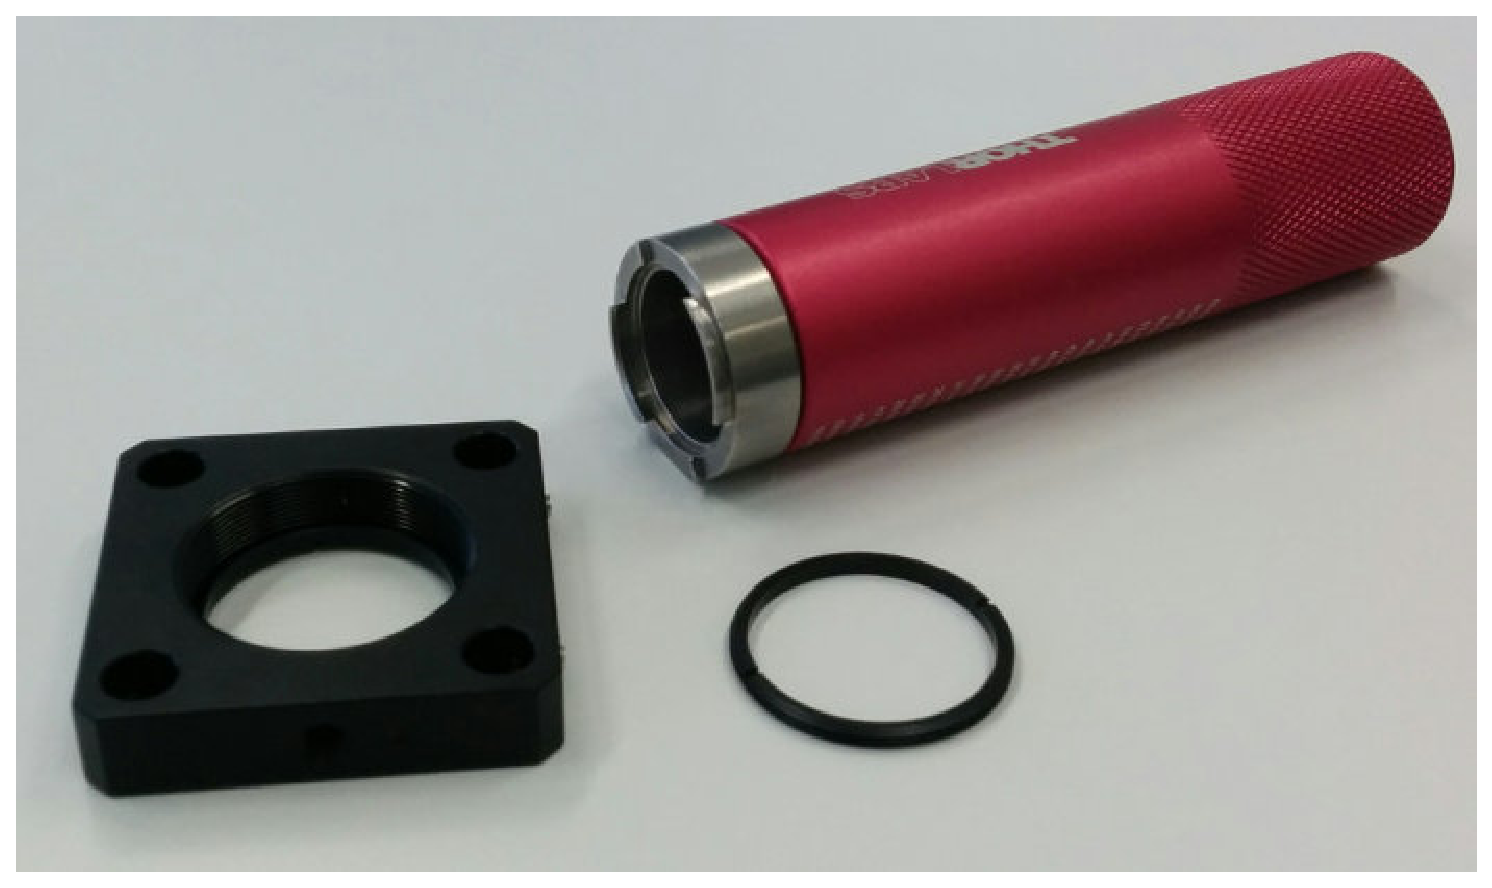
\includegraphics[width=2in]{lens_tool.eps}
\caption{A post holder bolted to a rail carriage (left \& middle).
The lens tool secures lenses in the holders using the rings (right).}
\label{fig:post}
\end{figure}


\clearpage

\section{Image Formation}
An image is formed when all light rays leaving one point (or region) of the object arrive at some other defined point (or region) \textit{regardless of the angle of the ray}. 
This is illustrated in Fig.~\ref{fig:imageforming}, where the grey mouse on the left is imaged through a lens to form an inverted image: the green mouse on the right. 
All light rays leaving the grey mouse's left ear converge onto the inverted image's left ear. 
When we put a sheet of paper in the image plane, we see points on the paper illuminated by rays coming from corresponding points in the object. 



\begin{figure}[h]
\center
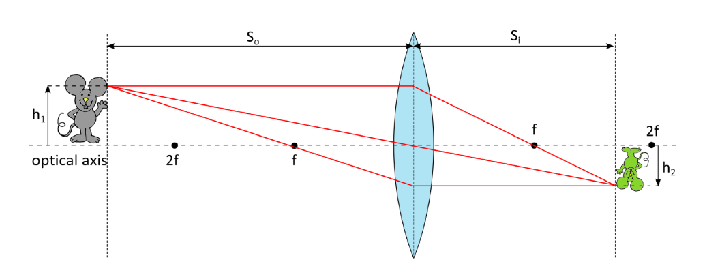
\includegraphics{image_forming_basics.eps}
\caption{Simple image formation using one lens. 
The focal length of the thin lens is $f$, object distance is $s_o$ and image distance is $s_i$. 
The upper ray (parallel to the optical axis on the left) passes through the focal point (denoted as a dot) on the right side of the lens, the middle ray (passing through the centre of the lens) is unrefracted, and the lower ray passes through the focal point on the left side of the lens, and comes out parallel to the optical axis on the other side. 
}
\label{fig:imageforming}
\end{figure}

As the distance between the object and lens ($s_o$) is varied, the distance between the lens and image ($s_i$) also changes. This relationship is determined by the lens focal length ($f$) using the thin lens equation.

\begin{equation}
\frac{1}{s_o} + \frac{1}{s_i} = \frac{1}{f}
\label{eq:thinlens}
\end{equation}

The following conventions are used: $f>0$ for convex lenses, $f<0$ for concave lenses, $s_o$ is always $>0$, $s_i>0$ for real images, and $s_i<0$ for virtual images.
Transverse distances above the optical axis are $>0$. Distances below are negative. 

\vspace{2.5em}
You will need to get comfortable with drawing ray diagrams, since you will do this later to explain what you observe on the bench.
Copy the diagram in Fig.~\ref{fig:imageforming}.
Draw the three cardinal rays:
\begin{itemize}
\item The ray parallel to the optical axis goes through $f$ on the image side.
\item The ray that passes through the centre of the lens travels undeflected.
\item Finally, the ray that goes through $f$ on the object side leaves the lens parallel to the optical axis on the image side. 
\end{itemize}


\clearpage




\subsubsection{1. Determine the focal length of a convex lens }
For the next few exercises you will use an LED as both a light source and an object to image.
You will form various images of the LED emitter. 
Your first task is to set up the LED on the optical rail:

\begin{itemize}
\item Attach a post holder to a rail carriage (Fig.~\ref{fig:post}) and place this on the rail. 
\item Place the LED in the SM1 holder and attach this to a cage plate (CP02) and mount this on a 50~mm post. 
\item Mount the post to your post-holder and place the LED at one end of the rail.
\item Power the LED (remembering to use the current-limiting resistor). 
\end{itemize}


Now choose a lens with a focal length of about $f=100~mm$ and attach the lens to a lens holder using the lens wrench and a retaining ring (this should already be in the lens holder).
Mount the lens on another carriage and attach to the rail next to the LED. 
Get the LED aligned with the middle of the lens (precise alignment isn't important). 

You will use this lens to form an image of the LED.
This is called \textbf{finite conjugate} imaging because the image is paired (i.e. conjugated) with an object at a finite distance from it.
The image and sample planes are said to be \textbf{conjugate planes}.
You will be able to form an image on a piece of card or paper if the distance between the lens and LED ($s_o$) is $>1f$.
The image will be of the LED emitter, which  usually looks like a small bright square, often with fine lines going across it. 
If all you see is a blur, you have not formed an image.

\begin{itemize}
\item Place the lens $<1f$ from the LED and use a piece of card on the other side of the lens to verify that no image is formed at any distance from the lens.
\item Why is no image formed? 
Hint: draw a diagram with the object at $<1f$. Plot just two rays: the undeflected ray and the ray coming out parallel with the optical axis and then going through $1f$ on the image side. 
How do the rays behave after they have passed through the lens?
\item Verify that an image is formed when the lens is $>1f$ from the LED: place a card very far from the LED (e.g. at $10f$ or $20f$) and slowly move the lens away from the LED. 
What is the distance between the LED and the lens at which you see an image? 
It should be just over $1f$.
\item Measure $s_i$ for three values of $s_o$ and fill in the table below. 
Using equation~\ref{eq:thinlens}, calculate $f$ for each value of $s_o$.
\item What is the value of $s_i$ when $s_o=2f$?
\end{itemize}

\vspace{2em}
\begin{tabular}{| p{1cm} | p{1cm} | p{1cm} |}
\hline
 $s_o$  &  $s_i$  &  $f$  \\
\hline
\hline
 & & \\ \hline
 & & \\ \hline
 & & \\ \hline
\end{tabular}


\clearpage

\subsubsection{2. Magnifying the image}
As you probably noticed, the size of the image of the LED emitter varied with $s_o$.
A lens produces images of different magnifications depending on $s_o$; an image can always be formed when $s_o>f$. 
The magnification of a lens is calculated as follows:

\begin{equation}
M = \frac{h_i}{h_o} = -\frac{s_i}{s_o} = \frac{f}{f-s_o}
\label{eq:mag}
\end{equation}

A value of $M=1$ would mean unitary magnification (the image is the same size as the object). 
Negative numbers indicate an inverted image.

To begin thinking about magnification, hand-draw the ray diagram (as in Fig.~\ref{fig:imageforming}) for the smallest and largest values of $s_o$ that you used above. 
Make sure to give yourself plenty of room. 
Hint: You will run out of paper if you use values too close $1f$.
If you're stuck, choose $1.5f$ and $4f$.
Note the changing angles of the rays and how they lead to different image sizes as $s_o$ changes. 
We will now see what happens when the rays come from infinity:

\begin{itemize}
\item Mount a lens of about $f=60~mm$ in a holder and attach a post to it. 
Go over to the window and form an image of the outside world on a piece of paper. 
The image is formed at $1f$.
\item Repeat with a lens of about $f=100~mm$ lens. 
What two things do you notice about the image? 
\item Fig.~\ref{fig:outside} models the situation you saw. Satisfy yourself that this provides a reasonable explanation. 
\item Go back to the lens and LED.
Calculate the values of $s_o$ and $s_i$ which produce $M=-4$ (remember, negative just means inverted) for a $f=100~mm$ lens. 
Measure the size of the LED image and so calculate the size of the LED emitter. 
\item Remember the value of $s_i$ when $s_o=2f$? Therefore what is $M$ when $s_o=2f$?
\end{itemize}


\begin{figure}[h]
\center
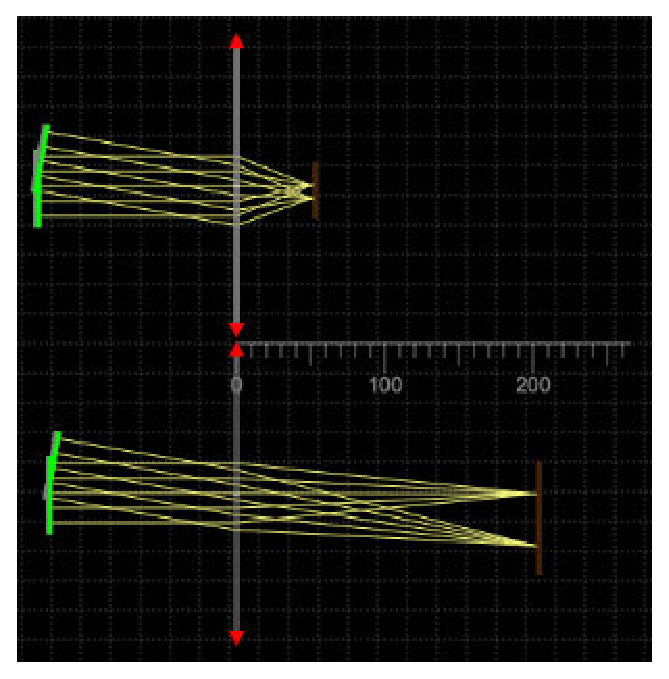
\includegraphics[width=2.5in]{image_forming_outside.eps}
\caption{Images formed at $1f$ from light originating at infinity. 
The top is a $f=50~mm$ lens and the bottom a $f=200~mm$ lens.
Light from different regions of the object arrive in parallel rays that come in at different angles. 
Each set of parallel rays come into focus at a point, satisfying the image-forming condition. }
\label{fig:outside}
\end{figure}


What you have covered above demonstrates an important property of lenses: that they work the same both forwards and backwards.
Recall the definition of an image-forming condition: \textbf{light rays leaving one point (or region) of the object arrive at some other defined point (or region)}.
This is why no image was formed when the LED was at $s_o=f$, since rays leaving the lens are parallel and do not converge on the other side. 
However, you \textit{were} able to form an image at $s_i=f$ when the object was very far away. 
The ray diagrams of these two conditions are \textit{identical}--the only difference is that the object is at $1f$ in the first case and at infinity in the second case.

\clearpage


\subsubsection{3. Virtual images}
At distances $s_o<f$, you were unable to form an image of the sample on the card because the rays emerging from the other side \textit{diverged}.
\begin{itemize}
\item Place the LED at $0.5f$ from a lens of your choice, observe the light diverging as it exits the lens.
\item Draw the ray diagram for this $0.5f$ scenario:
Draw the ray that leaves the tip of the object and continues undeflected through the middle of the lens. 
Draw the ray that travels parallel to the optical axis and goes through $1f$ on the other side.
See how these rays diverge. 
\end{itemize}

It would seem that no image is formed yet, surprisingly, a \textit{virtual image} is formed on the same side of the lens as the object. 
This may sound like a peculiar concept, but you are already familiar with virtual images as this is how you see images in flat mirrors (Fig.~\ref{fig:mirror}). 
The extended rays in the case of the mirror can be created from the \textit{diverging} rays from the object. 
In the case of the the lens at $s_o<f$ we also have diverging rays and so can also draw extended rays as we did for the mirror. 
Add the extended rays to your ray diagram by continuing the rays on the object side of the lens until they converge. 
A virtual image is formed where they converge.
What does your diagram tell you about the magnification of the virtual image?
Verify this: pick up the lens, place it $<1f$ from an object and look through it.
\begin{figure}[h]
\center
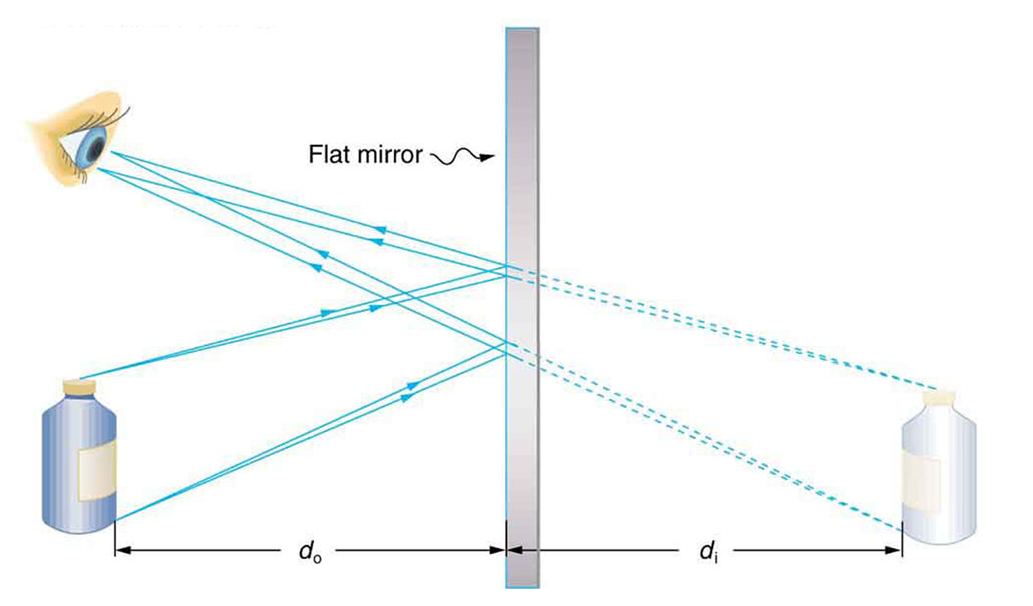
\includegraphics[width=4in]{virtual_image_mirr.eps}
\caption{A virtual image of the bottle is created on the far side of the mirror. 
This is described by the dotted lines which are `extended rays' that are used to form the virtual image. }
\label{fig:mirror}
\end{figure}

A virtual image is also formed by a negative (concanve) lens, as shown in Fig.~\ref{fig:neglens}. 
Examine the ray diagram of the negative lens. 
What do you predict you will see if you look through a negative lens?
Verify this with the $f=-50~mm$ lens.
\begin{figure}[h]
\center
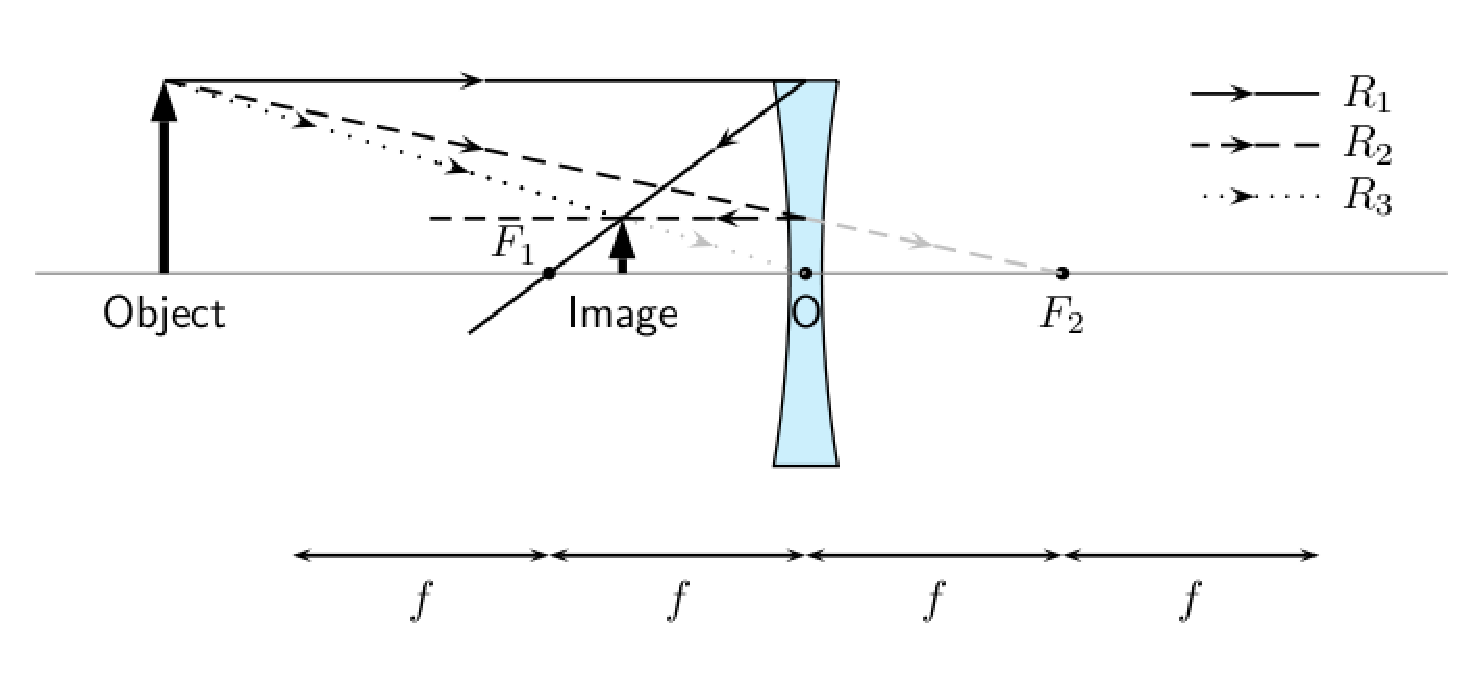
\includegraphics[width=3.5in]{negative_lens.eps}
\caption{Ray diagram of a negative lens.}
\label{fig:neglens}
\end{figure}

In summary, a \textbf{real image} is formed on the opposite side of the lens to the sample. 
This allows the detector to be physically separated from the sample, which is rather useful.
A \textbf{virtual image} is formed on the \textit{same} side of the lens as the object. 

\clearpage

\subsection{Infinite Conjugate}
The \textbf{infinite conjugate} refers to the situation where the object is located at a distance of $1f$ from a lens (Fig.~\ref{infiniteConjugate}). 
In this scenario the rays leaving the lens are parallel and do not converge, so this is not an image forming condition. 
Instead, the image can be considered to be infinitely far away (hence the name). 
If a second lens is added, then an image can be formed. 
The magnification of the image is defined as Eq.~\ref{eq:magIC}. 
This arrangement is useful because the image is always formed at $1f$ from the second lens irrespective of the distance between the lenses.
Most microscope objectives are designed to work in this configuration since it allows filters to be added into the infinite space without altering the location of the image plane. 
Such objectives are known as `infinity corrected`, since they are designed to produce their best images with the sample at $1f$.

\begin{equation}
M=-\frac{f_2}{f_1}
\label{eq:magIC}
\end{equation}

\begin{figure}[h]
\center
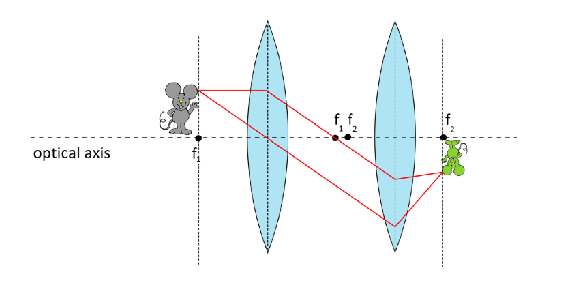
\includegraphics[width=4in]{infiniteConjugate.eps}
\caption{The infinite conjugate.}
\label{infiniteConjugate}
\end{figure}

\begin{itemize}
\item Set up two lenses with different focal lengths on the rail to build the infinite conjugate. 
Ensure that the first lens is at $1f$ from the LED before placing the second lens. 
\item Place a screen at the $f$ of the second and hold it in place with the post-mounted clip.
\item Verify the consequences of the infinite space by moving the second lens and maintaining the screen at $f$ of the second lens. 
What happens to the image size?
\item Swap the first lens with one of a different focal length. 
Verify that the image size changes in the manner in which you expect. 
\end{itemize}



\clearpage


\subsection{Beam expanders}
Lenses can be used to expand the diameter of a light beam, such a laser.
Expanders can be built using either two convex lenses (Fig.~\ref{beamExpander1}) or a convex and concave lens (Fig.~\ref{beamExpander2}). 
In both cases the lenses are set up such that their focal points coincide (i.e. they are separated by the sum of their focal lengths). 
The image formed by the first lens is imaged at infinity by the second lens.
The degree to which a beam is expanded is given by:
\begin{equation}
\frac{d_2}{d_1}=\frac{f_2}{f_1}
\label{eq:beamExp}
\end{equation}

\begin{figure}[h]
\center
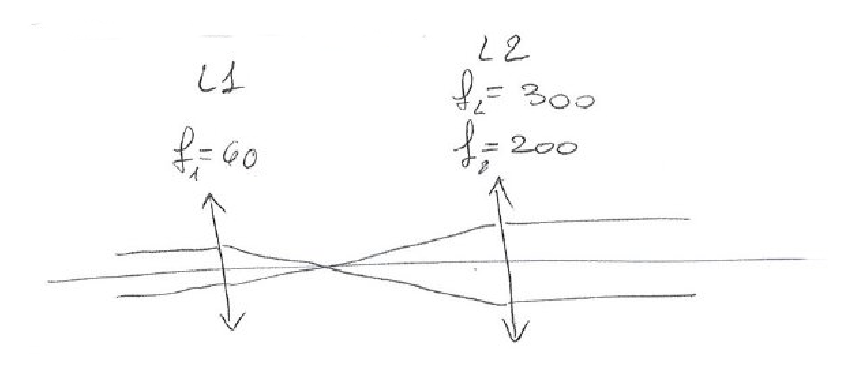
\includegraphics[width=4.5in]{beamExpander1.eps}
\caption{Beam expander with two convex lenses.}
\label{beamExpander1}
\end{figure}

\begin{figure}[h]
\center
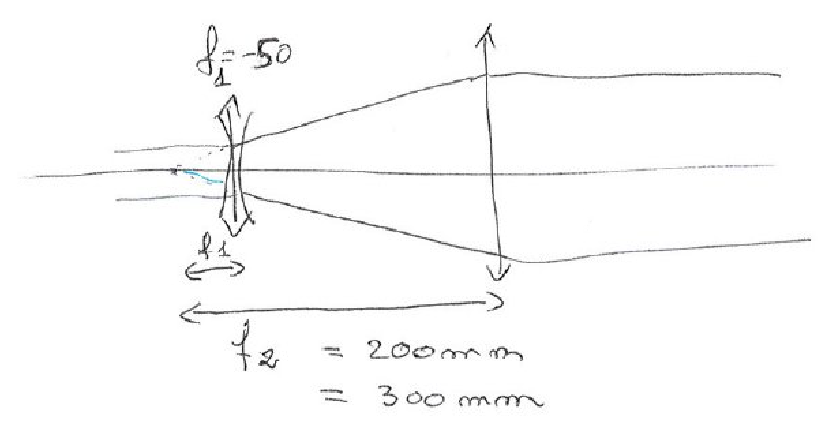
\includegraphics[width=4.5in]{beamExpander2.eps}
\caption{Beam expander with one convex and one concave lens.}
\label{beamExpander2}
\end{figure}

We need collimated light (parallel rays) entering the system, so swap the LED for a laser pointer.
You will clamp your laser pointer and align it to the rail (i.e. have the beam traveling parallel with the rail). 
The lenses will then be aligned with respect to the beam. 
This is an easy way of producing a well-aligned optical system and you will use it again later in the practical.
The procedure is as follows:

\begin{itemize}
\item Attach an RA180 clamp to a 75 mm post (the irises are mounted on 75 mm posts) and clamp the laser pointer to it (Fig.~\ref{fig:mounted_laser}).
\item Place the pointer at one end of the rail.
\item Place the iris next to the laser pointer, close it and adjust the height of the laser pointer so the beam goes through the hole. 
\item Slide the iris to the other end of the rail. 
\item \textit{Rotate} the post the laser pointer sits on and change the clamping force to \textit{tilt} the pointer until the beam goes through the iris. 
\textbf{Do not translate the laser pointer up and down.}
\item Slide the pointer back down the rail and confirm that the beam still passes through hole. 
If not, \textit{translate} the laser pointer's post up and down, then repeat the previous step.
\end{itemize}

\begin{figure}[h]
\center
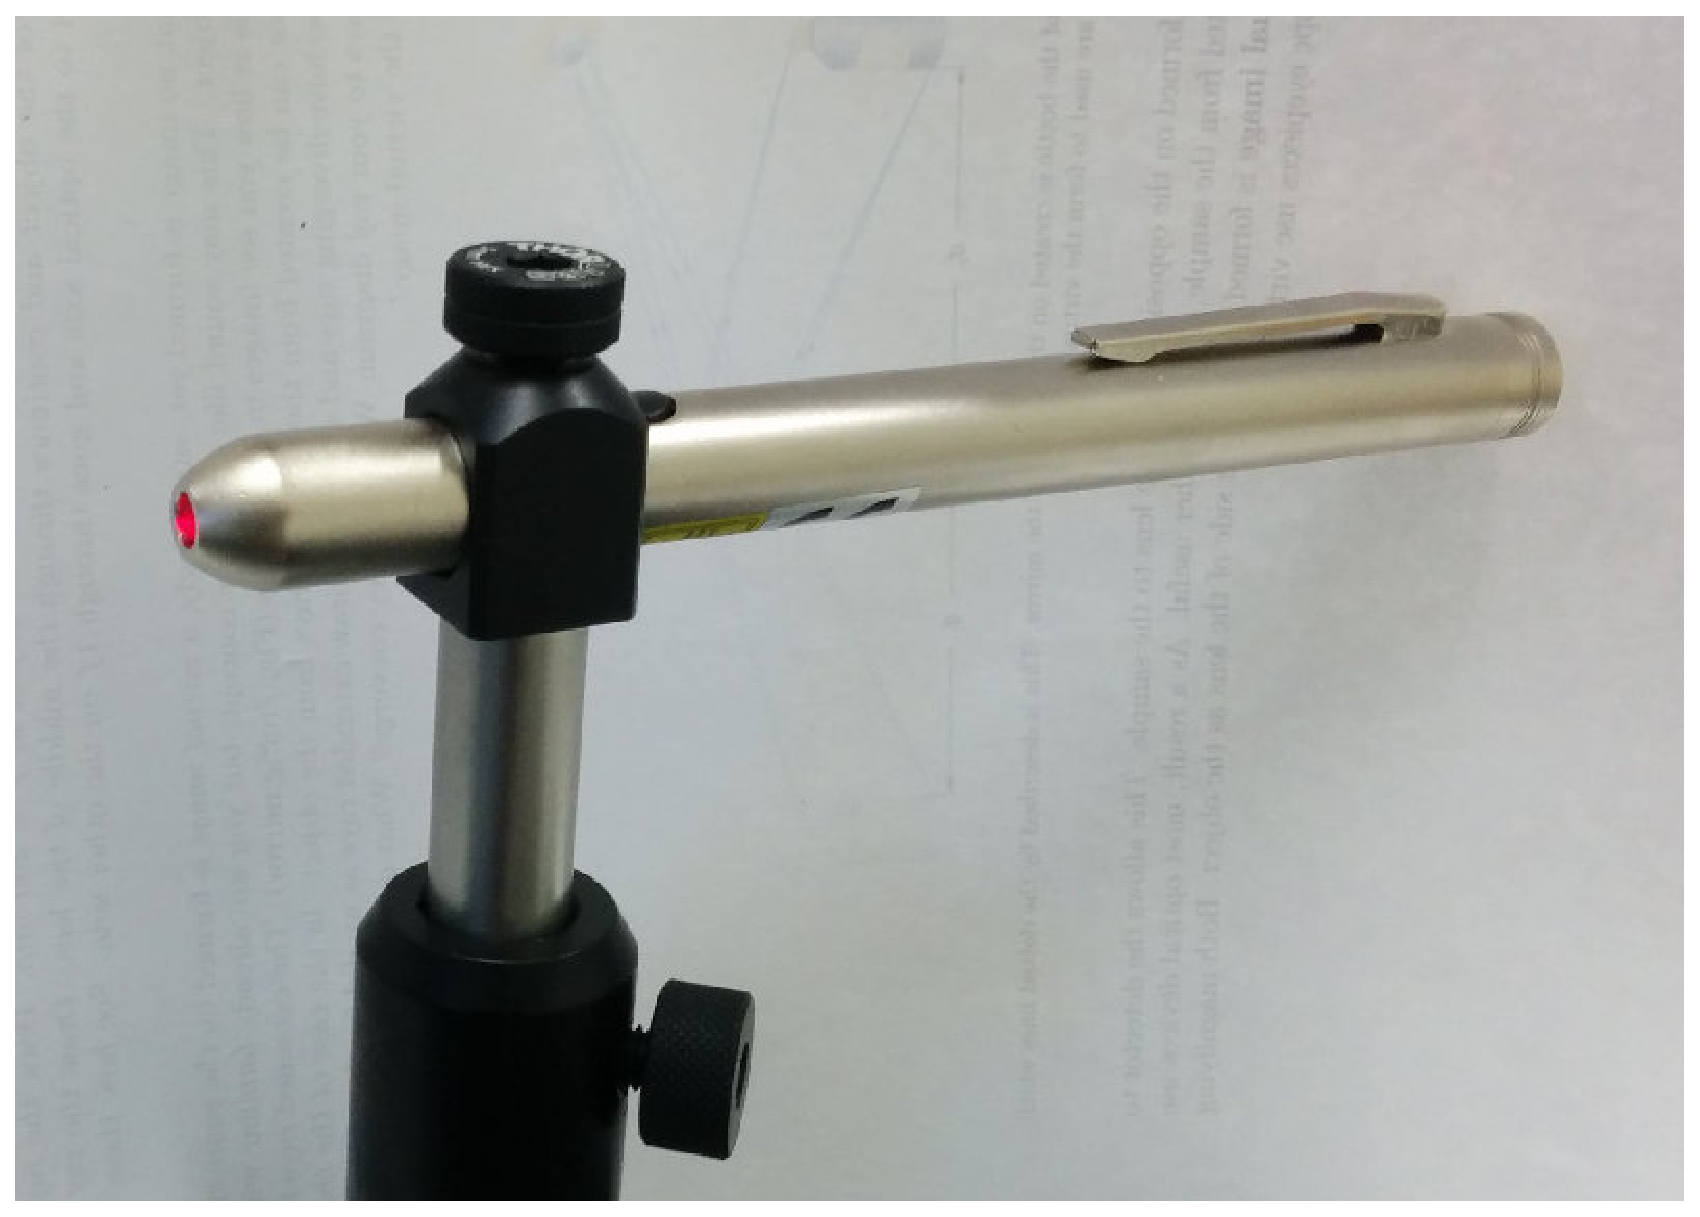
\includegraphics[width=3in]{mounted_laser.eps}
\caption{Laser mounted on a post.}
\label{fig:mounted_laser}
\end{figure}


Now you will build a 3x beam expander $f=300~mm$ lens and an $f=100~mm$ lens. 
These will be placed at the sum of their focal lengths and the laser pointer will be used as a guide for placing the lenses. 

\begin{itemize}
\item Place two more rail carriages onto the rail, between the iris and the laser pointer. 
\item Place the $f=100~mm$ lens onto the post carriage nearest the laser and position the iris roughly $1f$ from the lens.
\item You will know the lens is at the correct height because the beam will hit the middle of the iris. 
If you look carefully at the lens surface, you can also judge the height by looking at the back-reflection of the beam on lens surface. 
\item Slide the iris down the rail and complete the expander with the $f=300~mm$ lens. Again, use the iris as a target to judge lens height.
\item Make sure that the two focal points coincide by checking that the exit beam remains collimated (does not diverge or converge)
at all distances from the second lens. 
\item Measure the size of the expanded beam and so calculate size of the unexpanded beam.
\item Swap out the $f=100~mm$ lens with the $f=-50~mm$ concave lens. Verify that the expanded beam diameter doubles. 
What advantages does the negative lens add?
\item Build a beam expander to yield the maximum magnification your optics kit allows (e.g. $f=300~mm$ and $f=30~mm$ to yield 10x). 
The beam expander you have built also goes by another common name.  What is it? 
Hint: think about what happens to beams that do not travel on-axis (Fig.~\ref{fig:telescope}).
Once you've figured it out, remove the laser pointer and use your device. 
\end{itemize}


\begin{figure}[h]
\center
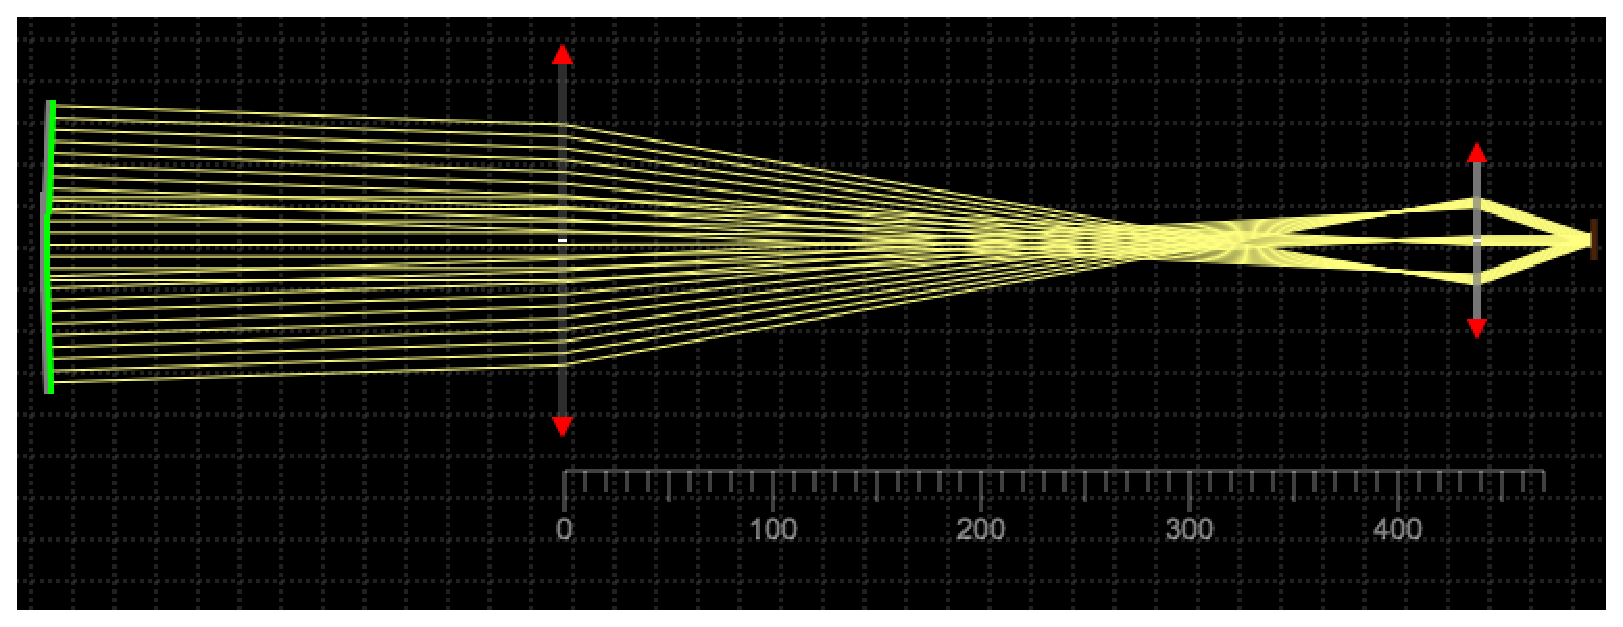
\includegraphics[width=4.5in]{telescope_ray_diag.eps}
\caption{A beam expander composed of an $f=400~mm$ lens and an $f=40~mm$ lens. 
In addition to the collimated beam arriving on-axis, two off-axis beams are shown.}
\label{fig:telescope}
\end{figure}

\clearpage



\subsection{Composite optical elements}
As you will have noticed above, image quality tends to be best in the centre of the field of view and decreases towards the edges. 
A variety of aberrations (Fig.~\ref{fig:aberrations}) are at play and these tend to become progressively worse for light coming in at steeper angles to the optical axis.

\begin{figure}[h]
\center
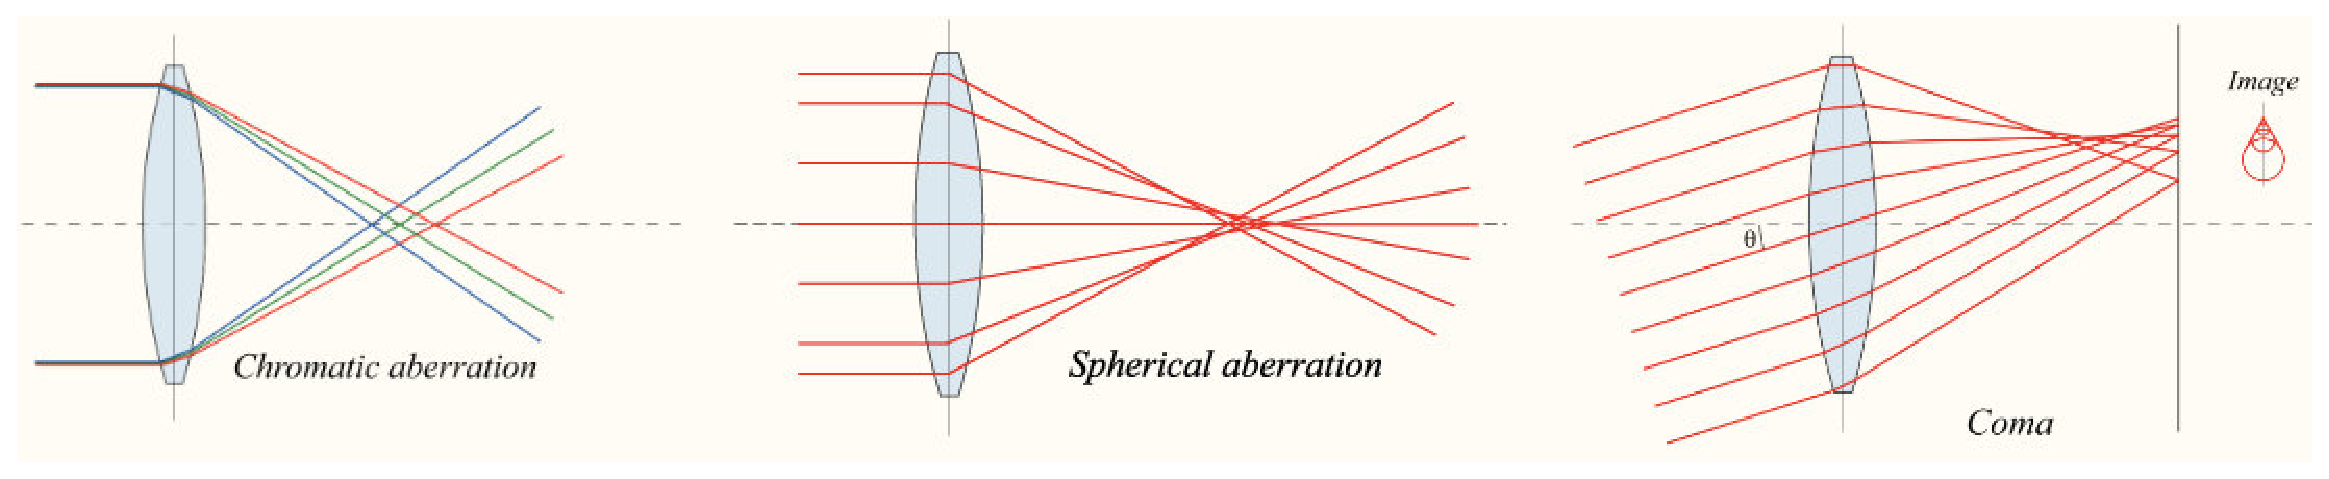
\includegraphics[width=6in]{aberrations.eps}
\caption{The three most common optical aberrations. 
Chromatic aberration sees light of different wavelengths coming into focus at different distances from the lens.
Spherical aberration sees on-axis light coming into focus at different distances from the lens. 
Coma is the situation where off-axis light does not come into focus in the same spot. }
\label{fig:aberrations}
\end{figure}

Aberrations are corrected in objectives and eyepieces (Fig.~\ref{fig:composite}) by combining optical elements with complementary aberrations. 
Note that in objectives and eyepieces the light doesn't pass through a focal point within the device and so they can be considered to be a single complex lens.

\begin{figure}[h]
\center
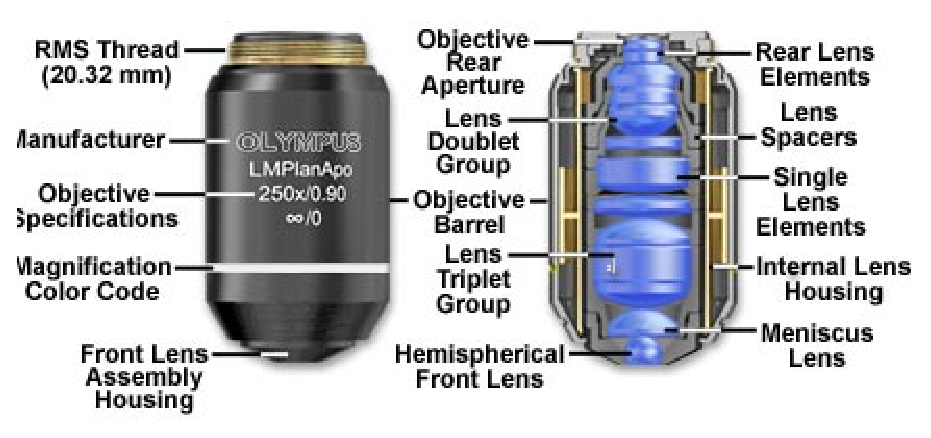
\includegraphics[width=2.8in]{objectivesfigure1.eps}
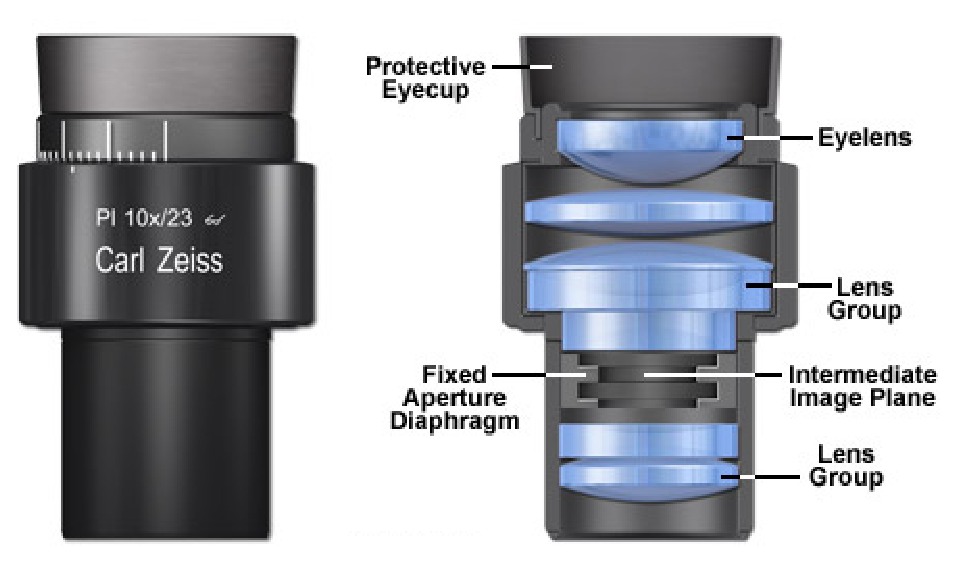
\includegraphics[width=2.2in]{eyepieces5.eps}
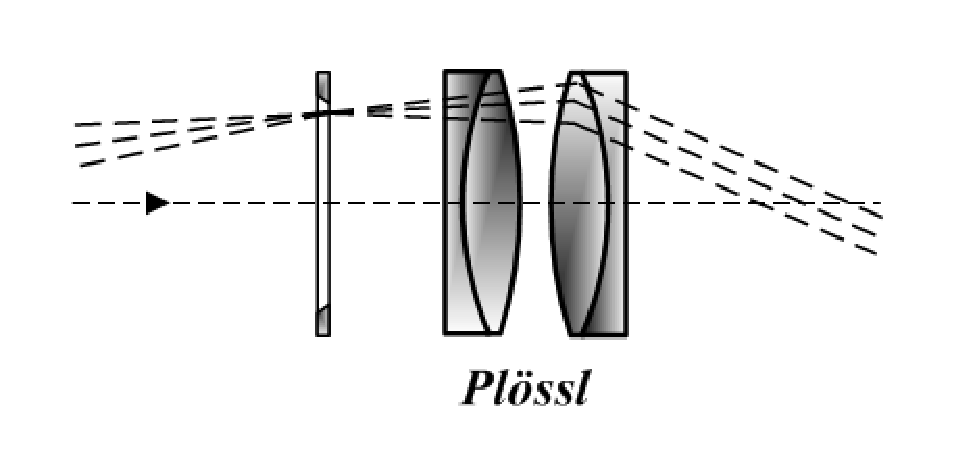
\includegraphics[width=2.2in]{Plossl.eps}
\caption{The composite lens arrangements found in microscope
  objectives (left) and eyepieces (middle).
  The Pl\"{o}ssl eyepiece is composed of two sets of achromatic doublet lenses (bottom).}
\label{fig:composite}
\end{figure}


Here we will experiment with a simple composite optical arrangement: the Pl\"{o}ssl eyepiece (Fig.~\ref{fig:composite}). 
Pl\"{o}ssls are commonly used in amateur astronomy because they are not expensive and provide a relatively wide (50 degree) field of view that is of good 
quality if the eyepiece is well made. 
Pl\"{o}ssls also make suitable scan lenses for two photon microscopy\footnote{Negrean \& Mansvelder, 2014, PMID: 24877017}.
You will now construct a Pl\"{o}ssl using two $f=60~mm$ singlet lenses.


\begin{itemize}
\item First construct a beam expander ($f_1$=30~mm lens and a $f_2$=300~mm). 
The expanded beam will be directed into your eyepiece, which will make it easier to measure its focal length.
\item Build the Pl\"ossl by placing the two $f=60~mm$ lenses as close as possible (with their flat sides facing outwards if you have plano-convex lenses). 
You might need to move the post holders on the rail carriages to allow the lenses to meet.
Since collimated light leaves your beam expander, you can place the Pl\"ossl at any distance from the $f=300~mm$ lens. 
\item Verify that your Pl\"{o}ssl behaves more or less as expected: 
Eq.~\ref{eq:compoundLensF} gives the distance between the middle of the compound lens and the focal point. 
\item Separate your lens elements by about 15~mm and measure and measure the change in focal length.
\end{itemize}

The effective focal length of two thin lenses separated in air by some distance $d$ is given by
\begin{equation}
\frac{1}{f} = \frac{1}{f_1} + \frac{1}{f_2} - \frac{d}{f_1f_2}
\label{eq:compoundLensF}
\end{equation}

A telescope built from two positive lenses is known Keplerian telescope. 
A Galilean telescope uses a negative lens as the eyepiece and forms a non-inverted image.
Build a Keplerian telescope using $f=300~mm$ singlet lens for the objective and a $30~mm$ lens for the eyepiece. 
Look through it familiarise yourself with what the image looks like then replace the eyepiece with your Pl\"{o}ssl. 
The magnification will be similar, but the image quality should be better: you'll get a wider apparent field of view and substantially less pincushion distortion. 
You will still see chromatic aberration. 
If you have an achromatic $f=300~mm$ doublet, then you can use this as the objective to get a reduction in chromatic aberration and a sharper image. 
Your telescope is powerful enough to see the moons of Jupiter. 


\subsection{Optics Challenge}
Arrange 4 lenses so as to form a de-magnified, real, upright
image. Hints: 
\begin{itemize}
\item Use one negative lens.
\item Space will be a problem: the lenses will take up the whole rail and so you will need to place the target and screen outside of the rail.
\item Use a bright light source to illuminate your target or the image will likely be dim. 
\item There are multiple solutions to this problem.
\end{itemize}


\clearpage
\section{Illuminating the sample}
Different samples are best illuminated in different ways.
In transmission microscopy, the sample is illuminated from the opposite side to which it is imaged. 
In fluorescence microscopy, the sample is illuminated from the same side, with the objective also serving as the condenser. 
It is not efficient to illuminate the sample directly (with no intervening lenses) because light is emitted in all directions from the source but only a narrow range of ray angles reach the specimen. 
In the following two exercises you will build two different illumination systems: critical and K\"{o}hler. 
You will be given a brighter light source (either a bright blue LED or a halogen light-guide).


\subsection{Critical illumination of a sample}
In critical illumination the light source is focused onto the specimen (Fig.~\ref{critIlum}).
A suitable sample is a coverslip with thin lines drawn on with a marker or you may use a specimen from the specimen kit, if you have one.
First you will set up critical illumination with one lens:

\begin{figure}[h]
\center
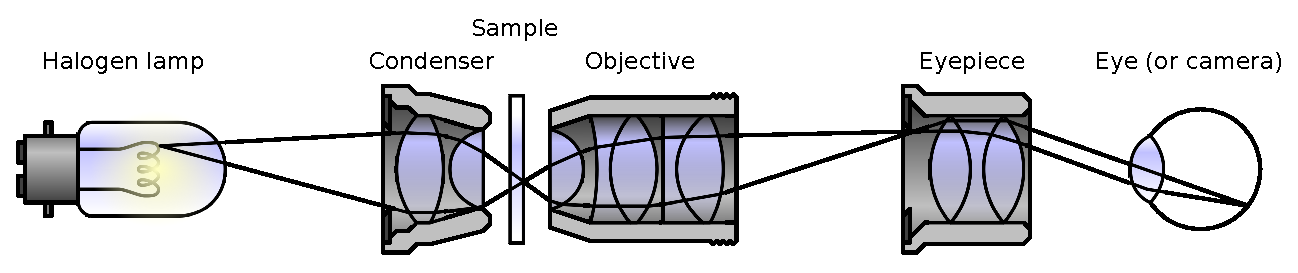
\includegraphics[width=5in]{Critical_Illumination.eps}
\caption{A simple critical illumination set up for visual microscopy.}
\label{critIlum}
\end{figure}


\begin{itemize}
\item Hint: to avoid running out of $50~mm$ posts in the exercise that follows, use $30~mm$ or $40~mm$ posts for the 2'' lenses, sample holder, and card holder.
\item Place the light source at one end of the rail and then put an $f=25~mm$ or $f=30~mm$ 1'' lens at $2f$ from it.
\item Place your sample at $2f$ on the other side, where the image of the LED emitter or fiber bundle is formed.
Note that you can place a glass slide in a DH1 card holder (the black clip) by removing a clip on one side and loosening the screws a bit.
\item Move the slide back and forth until an image of the LED emitter appears on it. Use paper to help you see this if needed.
\item Place the 4x objective after the slide. This objective has a working distance of about $20~mm$.
\item At the other end of the rail, place a viewing card onto which you will form an image.
\item Position an $f=200~mm$ lens $1f$ from the card. This is known as the tube lens and will image the sample onto the card
\footnote{The $f=200~mm$ lens will yield 4x. You could use the $f=300~mm$ lens if you wish, to yield 6x.}.
\item Move the objective back and forth a small distance to focus and obtain an image. 
\end{itemize}

The above arrangement is a simple microscope. 
As you might expect, the image of the sample also contains an image of the light source. 
This is obviously not ideal.
Before we go on to address this problem, let's improve the illumination by capturing more of the light from the source. 
The plan is as follows (don't build it yet):
We will add a $f=60~mm$ after the $f=30~mm$ lens, forming an infinite conjugate system. 
The lens nearer the source is known as the \textbf{collector lens} and will be at $1f$ from the source.
The lens nearer the sample is known as the \textbf{condenser lens} and is at $1f$ from the sample. 
This is still critical illumination, since the light source will be imaged onto the sample, but the collector lens will be closer to the source and so more light will be captured. We will align the lenses with the laser pointer:

\begin{itemize}
\item Remove all the posts (not the rail carriages) from the rail.
\item Add all 10 post and rail carriage assemblies to your rail. As you proceed, keep in mind that you will need 6 carriages between the objective and the light source.
\item Replace the light source with the laser pointer on a $75~mm$ post. 
\item Use an iris as before to align the beam. However, this time you will have to move it between post holders and maintain its height with an RA90 (90 degree clamp) 
attached to the iris post (Fig.~\ref{fig:clampedIris}) since you won't be able to slide it up and down the rail.
\item Replace the tube lens and position it at the same height as the beam. Use the iris to help you.
\item Add objective upstream of the tube lens. Get the laser beam hitting the middle of the of front element. 
\item Now place the iris in the specimen's post holder and locate the $f=60~mm$ condenser lens next to it, using the iris as a target. 
\item Replace the iris with the sample
\item Use the iris to place the $f=30~mm$ collection lens in front of the laser.
\item Leave the iris where it is but open it. 
\item \textbf{You should have two empty carriages between the iris and the condenser lens}
\item Replace the laser pointer with your light source. 
\item Move the lenses back and forth so as to obtain a focused image under critical illumination. 
\end{itemize}


\begin{figure}[h]
\center
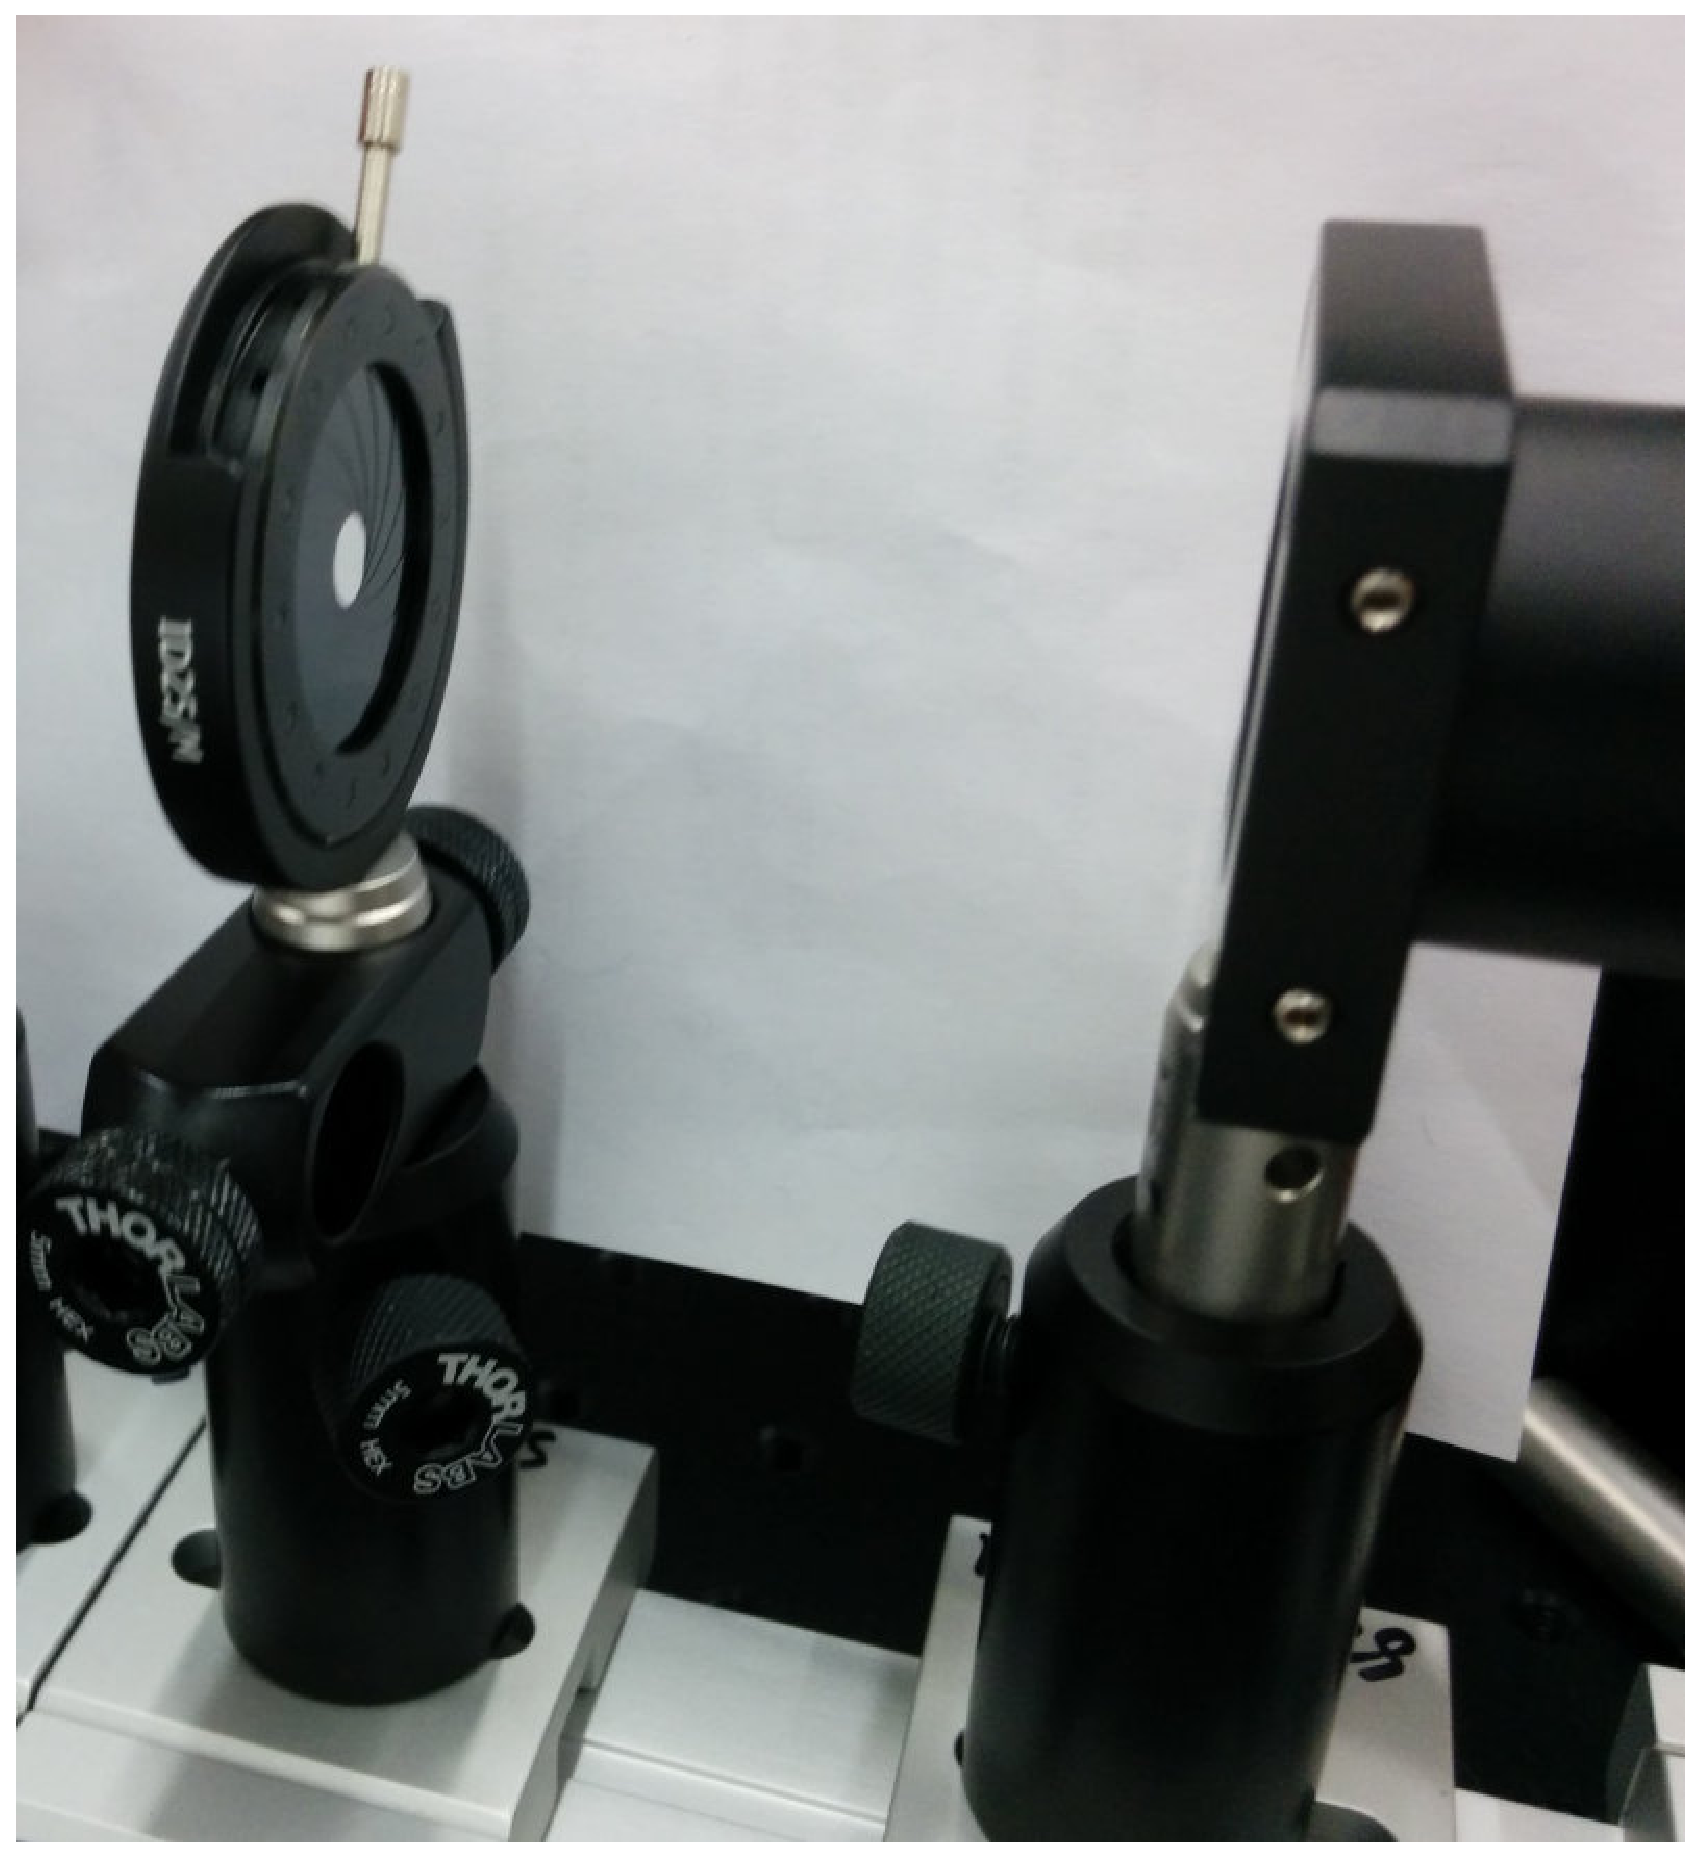
\includegraphics[width=3in]{clamped_iris.eps}
\caption{A clamp used to maintain the iris height so it can easily be moved between post holders}
\label{fig:clampedIris}
\end{figure}

With an infinite conjugate illumination system it becomes possible to regulate the NA of the illumination by varying the size of the iris in the infinite space. 
Try it!
By altering the NA of the illuminated light, the iris provides control over the resolution, contrast, and depth of field (Fig.~\ref{fig:critical_iris}).
To see the effect: open the iris, defocus slightly by moving the objetive, now close the iris. The image will go back into focus. 
You could also draw a cross on a coverslip with a marker and lay over your sample, then open and close the iris.

\begin{figure}[h]
\center
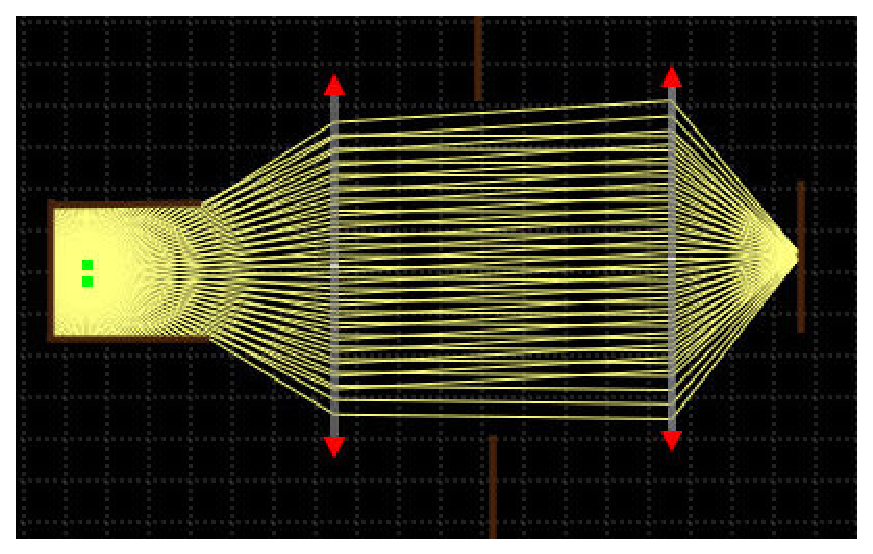
\includegraphics[width=2.8in]{critical_open_iris.eps}
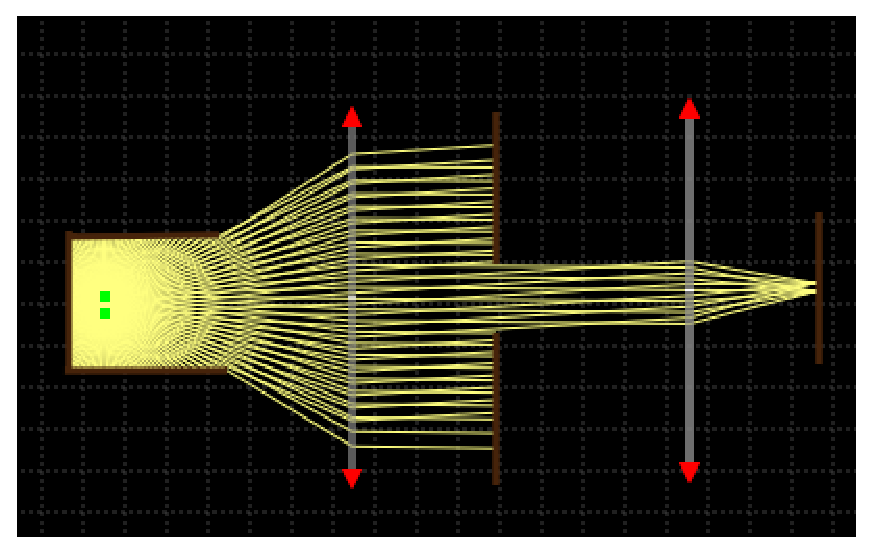
\includegraphics[width=2.8in]{critical_closed_iris.eps}
\caption{Critical illumination with two lenses. 
There is an iris after that collector lens that is open on the left image and closed on the right image. 
Note how closing the iris restricts the range of angles reaching the sample.}
\label{fig:critical_iris}
\end{figure}



\clearpage

\subsection{K\"{o}hler Illumination}
K\"{o}hler illumination is an important and commonly used technique in light microscopy, as it provides even illumination of the sample whilst ensuring the light source (e.g. the bulb filament) is not visible. 
This is achieved by adding a third lens, the field lens, before the condenser so that the image of the light source is out of focus at the sample. 
Since the source is out of focus, the illumination is uniform. 
Instead, the image is formed at $1f$ from the field lens. 
The condenser is then located at $1f$ from this image (as in a beam expander) so collimated (i.e. out of focus) light reaches the sample. 

The key to understanding K\"{o}hler illumination is to consider the two sets of conjugate planes in the system (Fig.~\ref{fig:koehler}). 
The \textbf{sample} is, of course, conjugate with the image plane but it also conjugate with a point $1f$ from the collector lens ($f_{CL}$ in Fig.~\ref{fig:koehler}). 
The \textbf{light source} is conjugate with a location between the field lens and the condenser ($f_F$ and $f_{CO}$ in Fig.~\ref{fig:koehler}). 
The light source is also conjugate with the objective back aperture (not shown in Fig.~\ref{fig:koehler}). 

\begin{figure}[ht]
\center
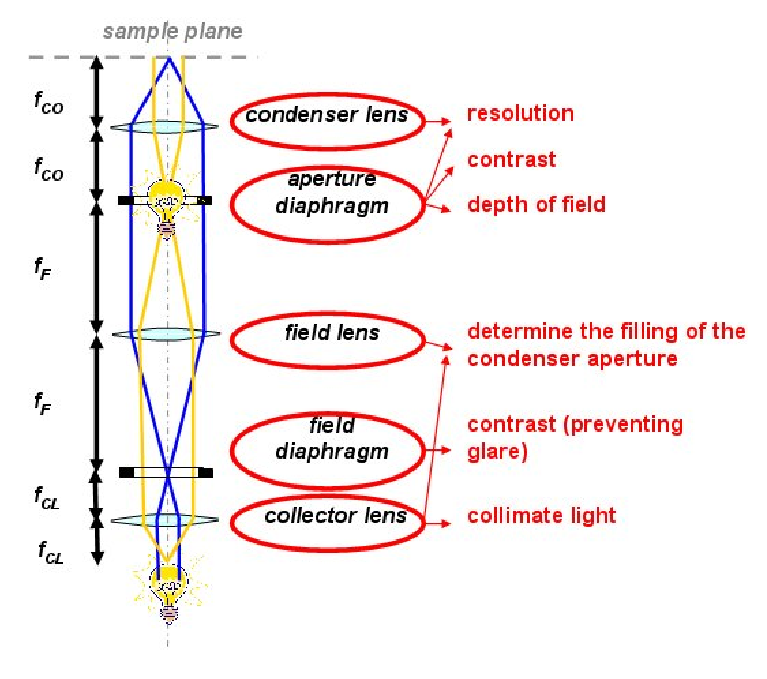
\includegraphics[width=5in]{koehler.eps}
\caption{K\"{o}hler Illumination. 
The blue lines indicate the conjugate relationship between the sample plane and the location of the field diaphragm.
The yellow lines indicate the conjugate relationship between the light source plane and the location of the aperture diaphragm.
}
\label{fig:koehler}
\end{figure}

At the the two conjugate planes in the illumination path are two irises (diaphragms). 
The \textbf{field diaphragm} is at $1f$ before the field lens, in the point conjugate with the sample. 
The field lens and condenser lens form an infinite conjugate system that image the field diaphragm onto the sample. 
The field diaphragm appears in focus at the sample and is used to regulate the area of illumination. 
This helps to improve contrast by minimizing stray light. 
Remember, the The \textbf{f}ield planes are the image \textbf{f}orming planes. 

The \textbf{aperture diaphragm} is located in the plane conjugate with the light source. 
i.e. it is located where an image of the light source is formed. 
Opening and closing this diaphragm regulates which regions of the light source can contribute to the illumination. 
Closing the diaphragm blocks off-axis regions of the light source and stops them from generating the more oblique rays that come out of the condenser. 
Closing the aperture diaphragm reduces the NA of the illumination and increases depth of field. 

\clearpage

You will now convert the critical illumination to K\"{o}hler illumination simply by adding the $f=60~mm$ field lens and an extra iris.
The components will be arranged in the following order and are all at $1f$ from each other (Fig.~\ref{fig:koehler}):
\begin{enumerate}
\setlength\itemsep{0.1em}
\item Collector lens
\item Field diaphragm.
\item Field lens ($f=60$)
\item Aperture diaphragm
\item Condenser lens ($f=60$)
\item The objective and tube lenses as before.
\end{enumerate}

The completed arrangement of the components is shown in Fig.~\ref{fig:koehler_completed}. 
Build the K\"{o}hler setup and observe that the image of the emitter is gone. 
You will likely need to tweak the distances between the components to get the field diaphragm conjugate with the sample. 
Once this is done, regulate the size of the field diaphragm and observe the effect. 
Defocus slightly and close the aperture diaphragm. Observe the effect.
You have finished! Unfortunately, the princess is another castle. See you tomorrow. 

\begin{figure}[h]
\center
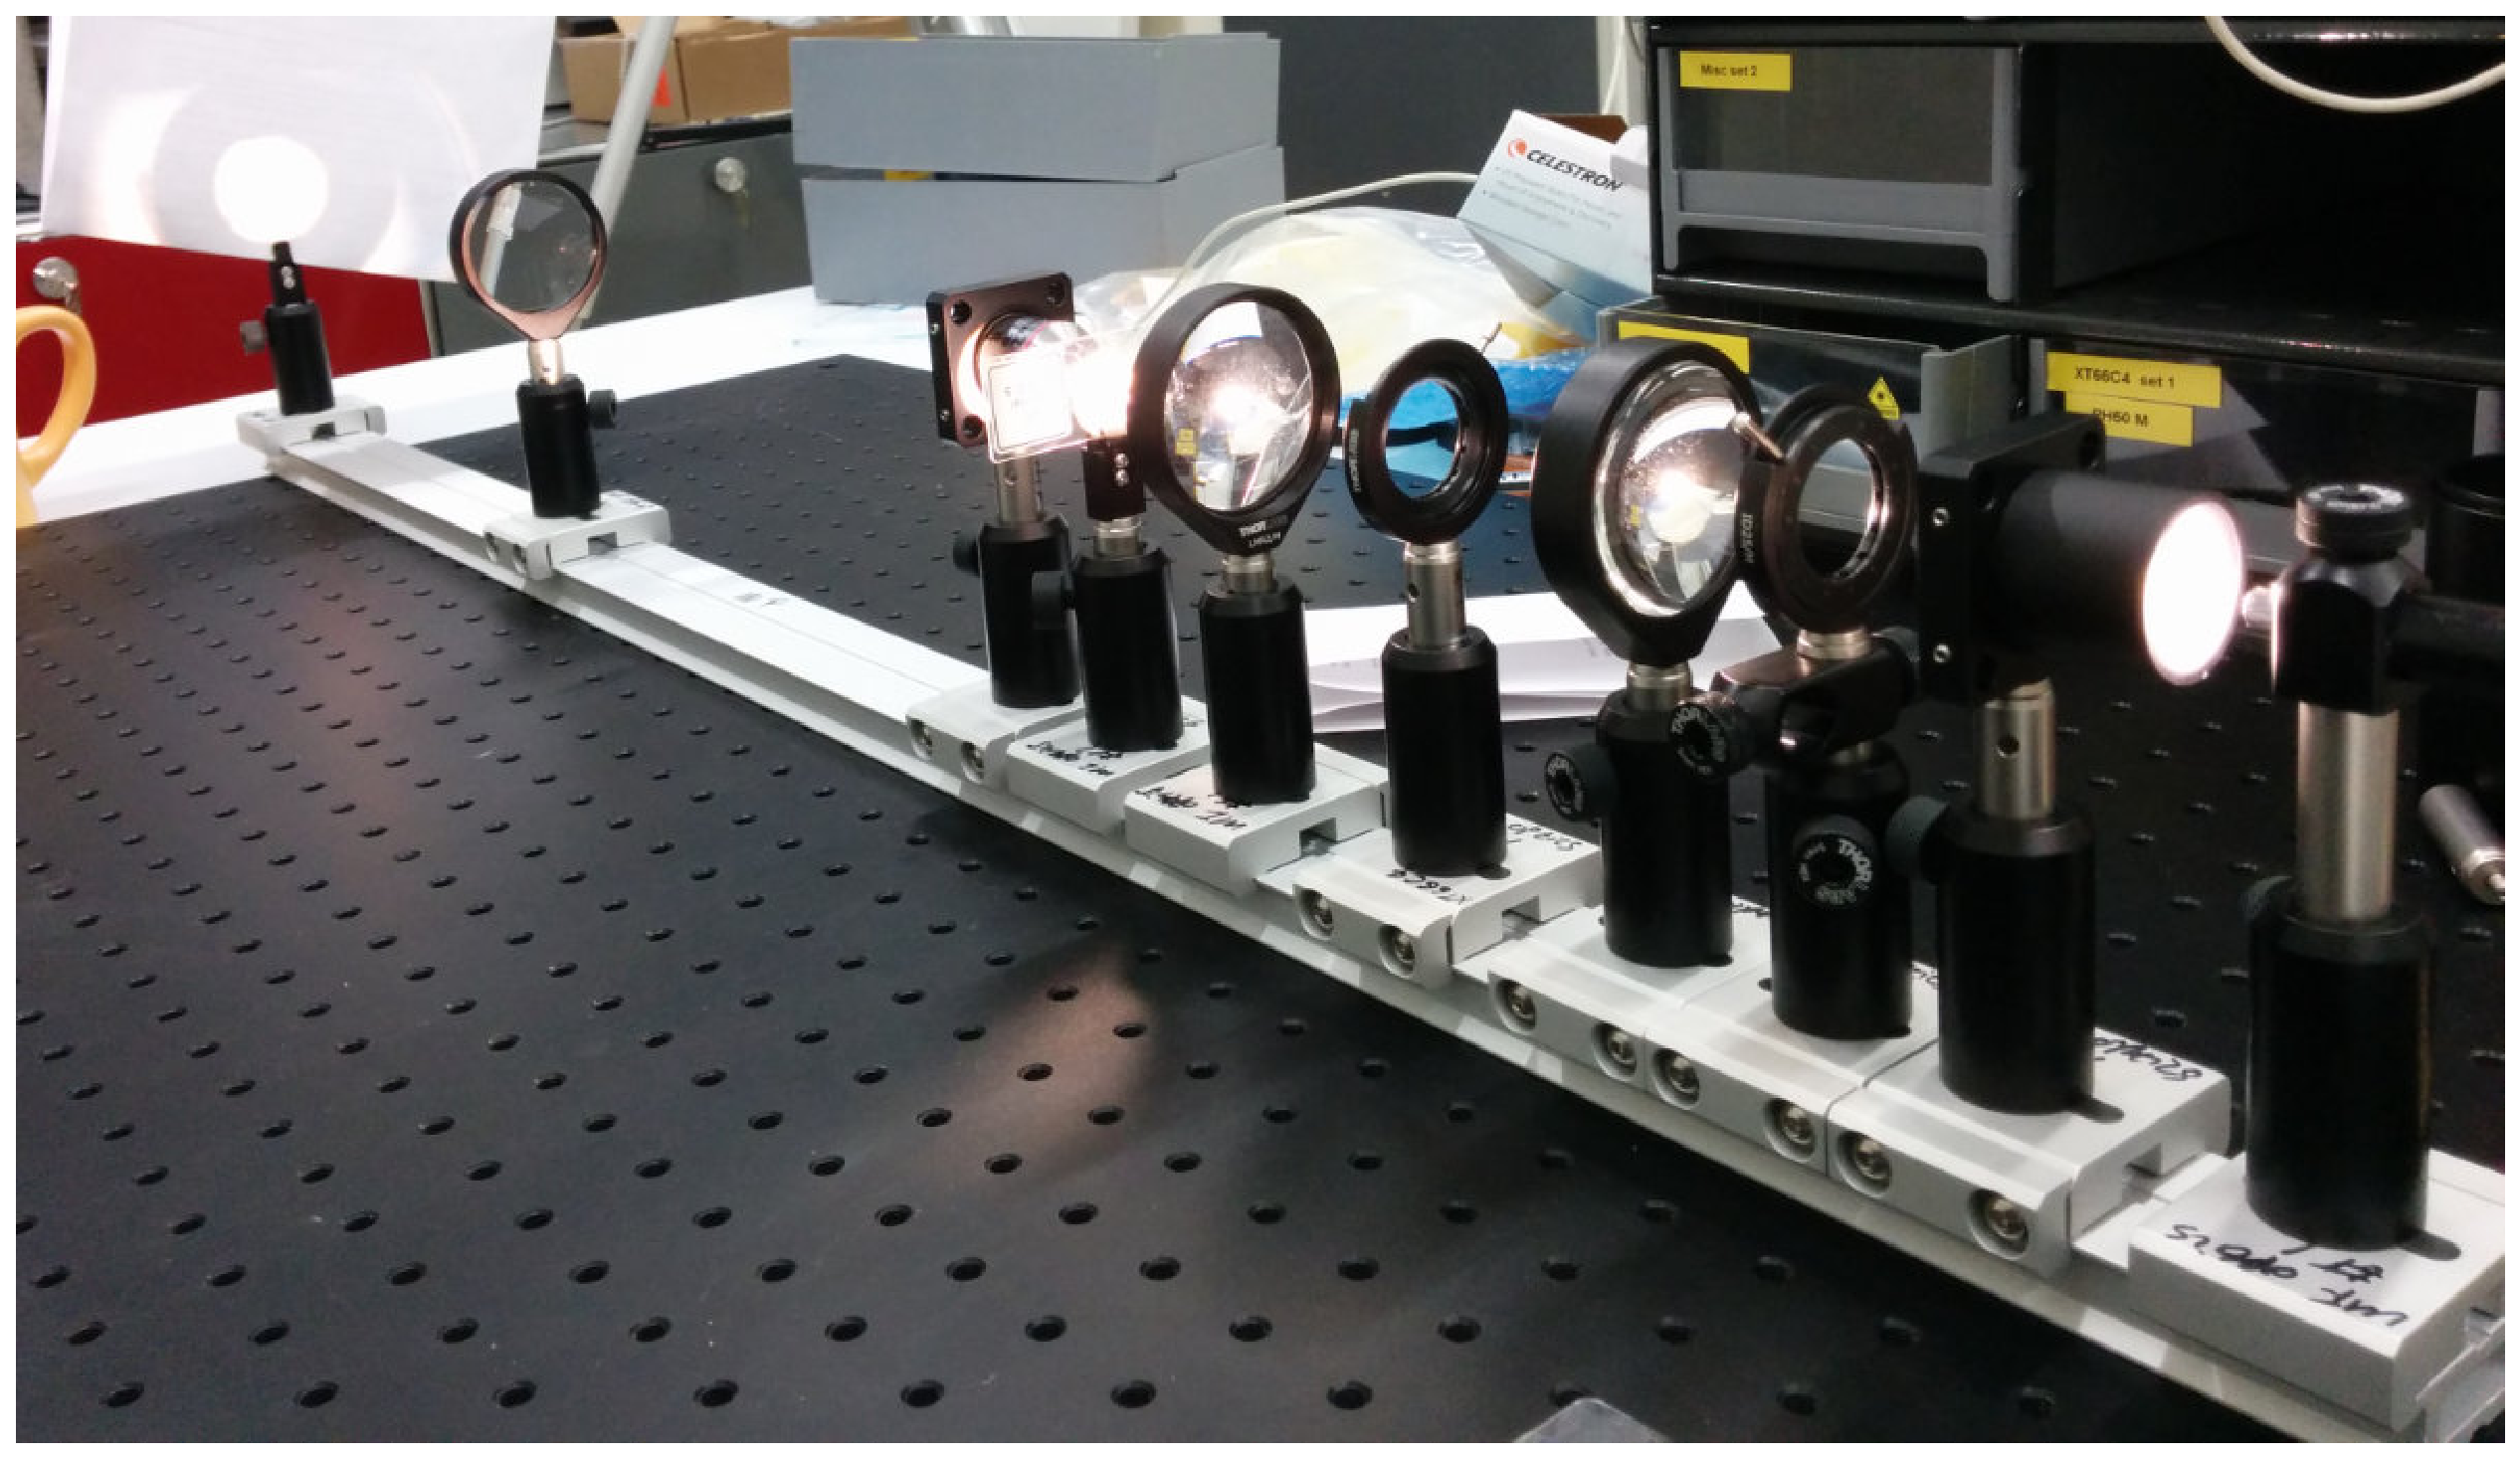
\includegraphics[width=5.5in]{illum_complete.eps}
\caption{The completed K\"{o}hler illumination assembly on a rail.}
\label{fig:koehler_completed}
\end{figure}






\end{document}
